\documentclass[runningheads]{llncs}
\usepackage{fontspec,xeCJK}
\setCJKmainfont{Noto Serif CJK SC}
\setCJKsansfont{Noto Sans CJK SC}
\usepackage{amsmath,amssymb,booktabs,graphicx,multirow}
\usepackage[hidelinks]{hyperref}
\renewcommand{\abstractname}{摘要}
\renewcommand{\keywordname}{关键词：}
\renewcommand{\figurename}{图}
\renewcommand{\tablename}{表}
\renewcommand{\refname}{参考文献}
\setlength{\emergencystretch}{1.5em}
\begin{document}
\title{事后之见并非机会：\\延迟反馈下风险约束标签获取的结果前价值}
\titlerunning{事后之见并非机会}
\author{匿名作者}
\authorrunning{匿名作者}
\institute{匿名机构}
\maketitle
\begin{abstract}
在信贷等决策系统中，标签需要通过有风险的行动获得，结果延迟到达，风险预算限制了可行的标签集合。获取策略常被拿来与事后最优集合比较，这会高估任何可部署策略实际能达到的效果。本文提出一套评价协议：把结果后提升空间分解为完全信息期望值（EVPI，即“先见”）项与结果前项；在结果概率已知时，用插值估计量与交叉拟合估计量从两侧夹住后者。借助一个由机制推导出的参照策略 DC-PRISM，我们得到四点发现：(i) 在待反馈信息具有方向性的受控世界中，十二种生成器变体下事后提升空间均有 82--88\% 可部署，且 DC-PRISM 在全部变体中都优于“数量最大化”的风险参照；(ii) 共同候选族上的消融表明，这一收益主要来自在以参照为锚的候选族上评估的目标加权信息代理，而非保守决策层；(iii) 先见在各种设定中大致恒定，约为 $1.5$--$6.4\times10^{-3}$ Brier，因此在可部署差异与之同量级的真实信贷协变量上，61--90\% 的事后提升空间属于先见，且对候选族大小不敏感；(iv) 在四个信贷队列上进行的、按统计功效设计的回放中，DC-PRISM 在两个队列上优于数量型参照，在另两个队列上不如信息贪心基线，实现风险远低于预算。
\keywords{选择性标签 \and 风险约束获取 \and 延迟反馈 \and 信息价值 \and 信用风险}
\end{abstract}

\section{引言}
\label{sec:intro}
放贷机构只能观察到自己批准的申请的还款结果，因此未来学习可用的数据取决于此前的决策~\cite{lakkaraju2017selective,wei2021selective}。每一次批准同时也是一次损失敞口，而结果要延迟一段时间才能到达。只要标签是用行动而不是标注工作“买来”的，以数据为中心的决策流水线就会面临同样的结构：风险预算、不完整的覆盖，以及已经承诺但尚未结算的信息。

主动学习与实验设计按观测对预测的期望贡献来选择观测~\cite{cohn1996active,chaloner1995bayesian,settles2009active}；近期的准则针对 Fisher 信息、预测信息或下游损失~\cite{ash2021fishing,bickfordsmith2023prediction,huang2026loss}。在风险预算下，一个信息量大但敞口高的观测可能挤掉好几个廉价观测，因此组成与数量之间直接权衡；待反馈结果又会改变这种比较，因为某些方向上的信息已经在路上。

在这种场景下应当如何\emph{评价}获取策略？常见的诊断做法是把所选集合与结果揭晓后表现最好的集合比较。这种比较混合了两样东西：策略本可利用手头信息实现的价值，以及必须知道隐藏训练标签才能获得的价值。在决策分析中，后者就是完全信息期望值（EVPI）~\cite{howard1966information,raiffa1961applied}；而在多个带噪估计中挑最优会产生向上偏差，即 optimizer's curse~\cite{smith2006optimizer}。这两点都不是新结论。缺少的是一套评价协议，使这种区分在风险约束获取中可以度量，并说明两部分在实际中各有多大。

\paragraph{贡献。}
\begin{itemize}
\item \textbf{评价协议。}把可见候选族上的结果后提升空间分解为 EVPI 型先见项与结果前项，给出后者的插值/交叉拟合夹逼估计，并表明所得占比对候选族大小稳定（第~\ref{sec:opportunity}、\ref{sec:controlled} 节）。
\item \textbf{机制。}同一状态下的数量—组成分解，以及一个双方向例子：在预算不变时，待反馈信息会使偏好集合发生反转。二者为设计提供依据，但实验并未单独分离出待反馈机制（第~\ref{sec:mechanism}、\ref{sec:controlled} 节）。
\item \textbf{分层证据。}在受控世界（含十二种生成器变体与决策规则的共同族消融）、带配对覆盖干预的真实信贷协变量，以及四个信贷队列上按功效设计的延迟回放（八个对照策略）中进行的预注册研究（第~\ref{sec:controlled}--\ref{sec:replay} 节）。
\end{itemize}
作为研究工具使用的 DC-PRISM 由该机制推导而来（第~\ref{sec:policy} 节）。我们不声称它在真实数据上优于简单的信息类基线；实验展示的是它在哪里有效、在哪里无效，以及它的哪些部分起作用。

\section{问题设定}
\label{sec:setting}
在第 $t$ 轮，学习者观察到有标签历史 $D_t$、待反馈获取的协变量 $O_t$、无标签候选池 $C_t$ 与目标协变量 $Q_t$。候选 $i$ 具有可见敞口 $e_i\geq0$ 与二元不利结果 $Y_i$，后者只在获取并经过反馈延迟之后才揭晓。合法策略只利用可见信息 $\mathcal H_t$ 选择 $S_t\subseteq C_t$；$O_t$ 与 $C_t$ 中的结果保持隐藏。学习效果用 Brier 分数~\cite{brier1950verification}度量。对固定状态，$L(S;Y)$ 表示在 $D\cup O\cup S$ 上拟合后的测试损失，其中 $Y$ 汇集了 $O$ 与 $S$ 的隐藏训练结果。

\paragraph{风险可行集合。}设 $q_i\in[0,1]$ 为选择时可用的风险分数，$\ell=\log(1/\alpha)$；当 $q\le1/2$ 时 $\phi(q)=q(1-q)$，否则 $\phi(q)=1/4$。对非空 $S$，
\begin{equation}
 R_\alpha(S)=\sum_{i\in S}e_iq_i+\Big(2\ell\sum_{i\in S}e_i^2\phi(q_i)\Big)^{1/2}+\frac{\ell}{3}\max_{i\in S}e_i,
 \label{eq:envelope}
\end{equation}
$R_\alpha(\varnothing)=0$，$\mathcal A_t=\{S\subseteq C_t:R_\alpha(S)\le B_t\}$。若在给定 $\mathcal H_t$ 时所选结果是 $p_i\le q_i$ 的独立 Bernoulli 变量，则次伽马界~\cite{boucheron2013concentration}给出 $\Pr\{\sum_{i\in S}e_iY_i>R_\alpha(S)\mid\mathcal H_t\}\le\alpha$。我们的分数不保证 $p_i\le q_i$，因此将式~\eqref{eq:envelope} 作为所有策略共享的操作性可行域，并以经验方式报告实际超出情况（第~\ref{sec:controlled}、\ref{sec:replay} 节）。

\paragraph{风险分数。}在 $D_t$ 上做 $\ell_2$ 正则逻辑回归得到 $\widehat\theta$。按拟合风险取 $D_t$ 的上半部分，令 $u$ 为其违约率的单侧 95\% Wilson 上界~\cite{wilson1927probable}，$\bar p$ 为该部分的平均拟合风险。把 logit 平移量 $\delta=\mathrm{clip}(\mathrm{logit}\,u-\mathrm{logit}\,\bar p,0.15,1.15)$ 加到 40 个 Laplace 抽样 $\bar x_i^\top\theta^{(m)}$（$\theta^{(m)}\sim\mathcal N(\widehat\theta,H_D^{-1})$）上，$q_i$ 取其 $0.9875$ 分位数的逻辑变换。

\paragraph{数量参照。}参照 $M_K\in\mathcal A_t$ 最大化集合基数，基数相同时取包络更小者；$K=|M_K|$。候选不超过 16 个时穷举。更大的池采用按敞口上限 $\max_{i\in S}e_i$ 分层的搜索：对每个不同的上限，分别排序均值与方差得到可行基数的上界，再用五种混合排序得到可行前缀，最后做降低包络的一换一交换。该过程对 $n$ 个候选耗时 $O(n^2\log n+nK^2)$，并在上界被达到时认证基数。在下文 1{,}408 个新离线状态中，有 1{,}320 个得到认证，包括 64 个“48 候选、$K=12$”池中的 63 个；其余 88 个（其中 85 个位于风险—信息负耦合的受控世界）中，上界比找到的基数多一个标签。

\section{机制与评价协议}
\label{sec:mechanism}
\subsection{数量与组成}
对 $|S|=k\le K$ 的所选集合，令 $M_k$ 为大小为 $k$ 的可行风险排序参照（$k=K$ 时沿用 $M_K$）。基于同一 $D\cup O$ 与实现结果，
\begin{equation}
\begin{gathered}
 Q_k=L(M_k;Y)-L(M_K;Y),\qquad C_k=L(M_k;Y)-L(S;Y),\\
 J=L(M_K;Y)-L(S;Y)=C_k-Q_k.
\end{gathered}
 \label{eq:decomposition}
\end{equation}
这个恒等式本身很初等，用途在于诊断。$Q_k$ 比较两个大小不同的风险参照，$C_k$ 比较大小相同的集合；因此 $J>0$ 且 $Q_k\approx0$ 时，收益应归因于组成，而非少取标签。

\subsection{方向性待反馈信息}
考虑一个双参数线性高斯模型，精度为 $P=\operatorname{diag}(h_1,h_2)$，目标权重为 $\operatorname{diag}(g_1,g_2)$，损失为 $\sum_jg_j/P_{jj}$。待反馈观测在方向 1 上增加精度 $o\ge0$；数量参照在方向 1 上增加 $a$，较小的备选在方向 2 上增加 $b$，二者均保持可行。备选的收益为 $J(o)=\frac{g_2b}{h_2(h_2+b)}-\frac{g_1a}{(h_1+o)(h_1+o+a)}$，关于 $o$ 严格递增；记 $v_2=g_2b/[h_2(h_2+b)]$，备选更优当且仅当
\begin{equation}
 o>o^*=\tfrac12\big(-a+\sqrt{a^2+4g_1a/v_2}\big)-h_1 .\label{eq:threshold}
\end{equation}
取 $h_j=g_j=1$、$a=4$、$b=1$、$\alpha=0.1$、$q=0.1$，参照每个标签敞口 $0.1$、备选敞口 $0.1624$，两种行动的包络均为 $B\approx0.2455$，且不存在可行的混合。$o=0$ 时参照更优（损失 $1.20$ 对 $1.50$），$o=1$ 时备选更优（$1.17$ 对 $1.00$），$o^*\approx0.464$。计算虽简单，却确定了一项设计要求：候选应相对于“历史加待反馈协变量”来估值。

\subsection{事后提升空间与结果前机会}
\label{sec:opportunity}
固定 $\mathcal H$，以及由可见信息构造、包含 $M=M_K$ 的有限集合族 $\mathcal F$。令 $\bar L(S;Y)$ 为对测试标签噪声积分后的 $L(S;Y)$，保留隐藏训练标签 $Y$。定义
\begin{align}
 H_{\mathrm{post}}&=\mathbb E\big[\bar L(M;Y)-\min_{S\in\mathcal F}\bar L(S;Y)\mid\mathcal H\big],\\
 H_{\mathrm{pre}}&=\mathbb E[\bar L(M;Y)\mid\mathcal H]-\min_{S\in\mathcal F}\mathbb E[\bar L(S;Y)\mid\mathcal H].
\end{align}
对任何在 $\mathcal F$ 内选择、期望收益为 $\Gamma_\pi=\mathbb E[\bar L(M;Y)-\bar L(\pi;Y)\mid\mathcal H]$ 的合法策略 $\pi$，
\begin{equation}
 H_{\mathrm{post}}-\Gamma_\pi=\underbrace{H_{\mathrm{post}}-H_{\mathrm{pre}}}_{\text{先见}}+\underbrace{H_{\mathrm{pre}}-\Gamma_\pi}_{\text{结果前选择差距}} .\label{eq:opportunity}
\end{equation}
先见项是隐藏训练标签对“在 $\mathcal F$ 中选哪个 $S$”这一决策的 EVPI~\cite{howard1966information,raiffa1961applied}；由 $\mathbb E\min\le\min\mathbb E$ 知其非负，且任何可部署策略都无法消除它。本文的贡献不在这个不等式本身，而在于把它用作评价协议：策略应当以 $H_{\mathrm{pre}}$ 为标尺；与实现最优集合比较的事后做法估计的是 $H_{\mathrm{post}}$，会恰好多算一个 EVPI，从而高估可部署机会。

\paragraph{估计。}当结果概率 $p$ 已知时，我们抽取 $R=128$ 组隐藏训练标签的重复样本 $Y^{(r)}$，用公共抽样在所有重复样本上评估每个 $S\in\mathcal F$。这样 $H_{\mathrm{post}}$ 的估计无偏。取重复均值最小者的插值估计 $\widehat H_{\mathrm{pre}}$ 因在噪声上做选择而向上偏，是 optimizer's curse 的一个实例~\cite{smith2006optimizer,cawley2010overfitting}。两折交叉拟合估计~\cite{chernozhukov2018double}在偶数重复上选 $S^\star$、在奇数重复上评估（反之亦然），向下偏。二者夹住 $H_{\mathrm{pre}}$，而 $H_{\mathrm{post}}-\widehat H_{\mathrm{pre}}^{\text{plug-in}}$ 是先见的保守估计。由于两项都相对于 $\mathcal F$ 定义，我们报告它们随 $|\mathcal F|$ 的变化（第~\ref{sec:controlled} 节）。

\section{DC-PRISM：由机制推导的参照策略}
\label{sec:policy}
DC-PRISM 用一个可行集合在历史与待反馈信息之上带来的目标加权 Brier 下降来为其估值，并与数量参照比较。记 $\bar x=(1,x^\top)^\top$、$p_\theta(x)=\sigma(\bar x^\top\theta)$、$w_\theta=p_\theta(1-p_\theta)$，令
\begin{gather*}
 H_{D+O}(\theta)=\Lambda+\!\!\sum_{i\in D\cup O}\!\!w_\theta(x_i)\bar x_i\bar x_i^\top,\qquad
 A_S(\theta)=\sum_{i\in S}w_\theta(x_i)\bar x_i\bar x_i^\top,\\
 W_Q(\theta)=\tfrac1{|Q|}\sum_{j\in Q}w_\theta(x_j)^2\bar x_j\bar x_j^\top,
\end{gather*}
以及
\begin{equation}
 V_\theta(S)=\operatorname{tr}\!\big[W_Q(\theta)\{H_{D+O}(\theta)^{-1}-(H_{D+O}(\theta)+A_S(\theta))^{-1}\}\big].\label{eq:value}
\end{equation}
$V_\theta$ 是目标 Brier 下降的局部二次代理，思路与转导式设计和预测信息获取一致~\cite{yu2006transductive,bickfordsmith2023prediction}；待反馈协变量不带标签地进入 $H_{D+O}$，这正是式~\eqref{eq:threshold} 中的折扣。

\paragraph{决策规则。}候选族 $\mathcal F_t$ 包含 $M_K$、按“价值/包络成本”排序的前缀、按价值排序的前缀，以及保留部分 $M_K$ 的交换集合，均按式~\eqref{eq:envelope} 检验可行性。对 $m=1,\dots,20$ 个抽样 $\theta^{(m)}\sim\mathcal N(\widehat\theta,H_D^{-1})$~\cite{mackay1992practical}，候选曲率按 $\exp[-0.45\{\bar x_i^\top(\theta^{(m)}-\widehat\theta)\}^2]$ 衰减；记 $a_m=\max\{V_m(M_K),10^{-6}\}$，
\begin{equation}
 Z(S)=\operatorname{quantile}_{0.2}\Big\{\tanh\frac{V_m(S)-a_m}{2.5a_m}\Big\}_m-0.22\,\frac{(K-|S|)_+}{\max(K,1)} .\label{eq:score}
\end{equation}
若 $Z>0.08$，DC-PRISM 选择 $\arg\max Z$，否则选择 $M_K$。我们把抽样分位数、曲率衰减、参照归一化、数量惩罚与门限统称为\emph{保守层}。这些常数沿用自软件包的早期版本，并在本文任何研究之前固定；我们无法证明它们的选取没有参考受控生成器，因此第~\ref{sec:controlled} 节对生成器和常数都做了扰动。构造候选族耗时 $O(Kn\,d^2)$，打分耗时 $O(20\,|\mathcal F_t|\,(d^3+Kd^2))$（$d$ 为特征数）；单核上 $n=24$ 时一次选择平均 53\,ms（最大 0.18\,s），$n=48$ 时 0.09--0.11\,s，贪心基线约 5\,ms。

\paragraph{对照策略。}所有策略共享状态、$q$、数值预算与式~\eqref{eq:envelope}。\emph{Safe-MinRisk} 返回 $M_K$。\emph{固定数量}按点价值选取 $K$ 的固定比例个标签。\emph{Fisher-cost} 按单观测参数方差下降与敞口成本之比贪心装填。另有四个基线贪心装填直到没有可行候选：\emph{Random}；\emph{Uncertainty}，按 $\widehat p(1-\widehat p)$ 排序~\cite{lewis1994sequential}；\emph{BAIT-greedy}，以池 Fisher 矩阵 $F_Q$ 对 $\operatorname{tr}(F_Q(H_{D+O}+A_S)^{-1})$ 做前向贪心~\cite{ash2021fishing}；\emph{TargetVar-greedy}，对式~\eqref{eq:value} 做前向贪心，是 EPIG 风格的 Laplace 近似~\cite{bickfordsmith2023prediction}，使用 DC-PRISM 的代理，但不用其候选族与保守层。贪心装填是背包型约束下此类目标的标准做法~\cite{krause2005near,sviridenko2004note}。

\section{受控证据}
\label{sec:controlled}
\paragraph{设计。}每个世界有 6 个特征、80 个覆盖较窄的历史标签、22 个待反馈获取、24 个候选、180 个目标点与 240 个测试点。候选分为低风险核心观测、与待反馈对齐的观测、另外两个预测方向上的观测，以及辅助尾部观测；后者的结果服从逻辑模型无法表示的状态切换。默认世界把全部待反馈获取放在同一方向上，并使信息与敞口正相关。所有选择在读取任何隐藏标签之前锁定。每项研究在运行前固定世界数、种子、比较族与 $5\times10^{-4}$ Brier 的实质效应阈值；协议与代码在执行前已在版本库中冻结（最后一批对应一个匿名提交哈希，列于补充材料）。我们报告配对均值、每个比较族内的 95\% Bonferroni 同时 $t$ 区间以及 Holm 校正检验~\cite{holm1979simple}；下文差值单位均为 $10^{-3}$ Brier。

\paragraph{实现收益及其组成。}在 128 个存档世界中，DC-PRISM 以 $3.27$ 个标签达到 Brier $0.1202$；Safe-MinRisk 用 6 个标签为 $0.1367$，取 $\mathrm{round}(0.75K)=4$ 个标签的固定数量规则也是 $0.1367$（配对超额 $16.49$，95\% CI $[10.97,22.00]$）。分解式~\eqref{eq:decomposition} 给出 $C_k=16.26$、$Q_k=-0.19$、$J=16.45$：收益来自组成，较小的风险参照并不比较大的差。

\paragraph{新世界，事前终点。}在 128 个新世界中，我们用期望 Brier 为每个策略打分：测试标签噪声精确积分，训练标签噪声用 128 组重复样本平均（表~\ref{tab:controlled}；此处固定数量取 $\lceil0.75K\rceil=5$ 个标签）。DC-PRISM 损失最低，其相对 Safe-MinRisk（$12.2$，$[7.6,16.8]$）、Fisher-cost、Random 与固定数量的收益均达到实质水平。相对 Uncertainty、BAIT-greedy 与 TargetVar-greedy 的收益为 $2.7$--$4.2$，区间含零。在另一组 128 个新世界（下文研究 F）中，DC-PRISM 相对 Safe-MinRisk 收益 $15.9$ $[8.5,23.3]$，相对 TargetVar-greedy 收益 $5.4$ $[1.0,9.9]$。

\begin{table}[t]
\caption{新受控世界（128 个）：事前期望 Brier、平均标签数，以及 DC-PRISM 的收益与 95\% 同时区间（$\times10^{-3}$；正值有利于 DC-PRISM）。}
\label{tab:controlled}
\centering\small
\begin{tabular}{lrrr}
\toprule
策略 & 期望 Brier & 标签数 & DC-PRISM 的收益 \\
\midrule
Safe-MinRisk & 0.1384 & 6.00 & $12.2$ [$7.6$, $16.8$] \\
固定数量 & 0.1358 & 5.00 & $9.6$ [$5.1$, $14.2$] \\
Random & 0.1359 & 3.54 & $9.7$ [$5.1$, $14.4$] \\
Uncertainty & 0.1304 & 2.81 & $4.2$ [$-0.8$, $9.2$] \\
Fisher-cost & 0.1440 & 2.67 & $17.8$ [$13.2$, $22.4$] \\
BAIT-greedy & 0.1289 & 2.22 & $2.7$ [$-1.3$, $6.7$] \\
TargetVar-greedy & 0.1290 & 2.19 & $2.8$ [$-1.2$, $6.9$] \\
DC-PRISM & \textbf{0.1262} & 3.12 & -- \\
\bottomrule
\end{tabular}
\end{table}

\paragraph{生成器扰动。}由于默认世界是围绕机制设计的，我们对其做了扰动（研究 G，每格 64 个新世界）：待反馈重叠程度 \{高, 中, 低\} $\times$ 风险—信息耦合 \{正, 中性, 负\}，用逻辑链接替换尾部状态切换，以及把候选池加倍到 48 个、分别取 $K=6$ 与 $K=12$。DC-PRISM 相对 Safe-MinRisk 的收益在全部十二格中都达到实质水平（$10.8$--$31.4$，表~\ref{tab:perturb}），包括没有误设尾部的世界和更大的候选池。相对 TargetVar-greedy 的收益在六个中性或负耦合格中的五个达到实质水平（$9.7$--$17.9$），其余七格（包括全部正耦合格）未定。各格中事后提升空间的结果前占比都在 82\% 到 88\% 之间。但受控收益并没有分离出第~\ref{sec:mechanism} 节的待反馈机制：待反馈重叠越低，收益反而越\emph{大}（高重叠 $11.5$--$16.9$，低重叠 $28.8$--$31.4$）；在此前的共同族研究中，从代理中去掉待反馈协变量只使损失变化 $0.9$ $[-1.0,2.8]$。因此，考虑待反馈信息只是一项设计依据，我们的证据既不能证实也不能否定它。

\begin{table}[t]
\caption{生成器扰动（每格 64 个世界；$\times10^{-3}$ 期望 Brier）。DC-PRISM 的收益及 24 项检验族上的 95\% 同时区间，加粗为达到实质水平；“结果前”为 $\widehat H_{\mathrm{pre}}^{\text{plug-in}}/H_{\mathrm{post}}$。}
\label{tab:perturb}
\centering\scriptsize
\setlength{\tabcolsep}{3pt}
\begin{tabular}{lrrrr}
\toprule
格（重叠 / 耦合） & 对 Safe-MinRisk & 对 TargetVar-greedy & $H_{\mathrm{post}}$ & 结果前 \\
\midrule
高 / 正（默认） & {\bfseries\boldmath $11.5$ [$4.7$, $18.4$]} & $4.6$ [$-0.1$, $9.3$] & 21.6 & 85\% \\
高 / 中性 & {\bfseries\boldmath $16.9$ [$7.6$, $26.2$]} & {\bfseries\boldmath $9.7$ [$3.1$, $16.2$]} & 26.6 & 87\% \\
高 / 负 & {\bfseries\boldmath $14.3$ [$6.9$, $21.7$]} & {\bfseries\boldmath $10.3$ [$3.3$, $17.3$]} & 21.7 & 86\% \\
中 / 正 & {\bfseries\boldmath $12.6$ [$4.0$, $21.2$]} & $4.5$ [$-1.2$, $10.2$] & 22.4 & 82\% \\
中 / 中性 & {\bfseries\boldmath $13.6$ [$5.5$, $21.6$]} & {\bfseries\boldmath $13.1$ [$4.9$, $21.2$]} & 23.4 & 83\% \\
中 / 负 & {\bfseries\boldmath $12.9$ [$1.1$, $24.7$]} & {\bfseries\boldmath $9.9$ [$2.8$, $17.0$]} & 22.3 & 83\% \\
低 / 正 & {\bfseries\boldmath $28.8$ [$16.3$, $41.3$]} & $3.8$ [$-3.6$, $11.2$] & 47.4 & 86\% \\
低 / 中性 & {\bfseries\boldmath $30.7$ [$17.6$, $43.8$]} & $7.2$ [$-2.3$, $16.8$] & 47.0 & 87\% \\
低 / 负 & {\bfseries\boldmath $31.4$ [$17.1$, $45.6$]} & {\bfseries\boldmath $17.9$ [$7.8$, $28.0$]} & 46.3 & 88\% \\
默认，无尾部状态切换 & {\bfseries\boldmath $10.8$ [$5.4$, $16.2$]} & $3.0$ [$-2.3$, $8.4$] & 19.9 & 84\% \\
默认，48 个候选，$K=6$ & {\bfseries\boldmath $14.9$ [$5.2$, $24.6$]} & $3.4$ [$-3.7$, $10.4$] & 24.0 & 87\% \\
默认，48 个候选，$K=12$ & {\bfseries\boldmath $12.5$ [$4.0$, $21.1$]} & $4.5$ [$-0.4$, $9.3$] & 21.0 & 88\% \\
\bottomrule
\end{tabular}
\end{table}

\paragraph{收益从何而来？共同族消融。}与 TargetVar-greedy 的比较把保守层与候选族混在了一起。因此在研究 F（128 个新世界）中，我们把各规则作用于同一个族 $\mathcal F^+$，即 DC-PRISM 的候选族加上 TargetVar-greedy 的集合。点代理自身的最大者 $\arg\max_{\mathcal F^+}V_{\widehat\theta}$ 相对 Safe-MinRisk 已有 $13.1$ $[6.1,20.2]$ 的收益；同一族上的完整保守层收益为 $16.1$，增量 $3.0$ $[-0.2,6.2]$，未得到证实。在保守层内部，用参数抽样而非仅在 $\widehat\theta$ 处计算式~\eqref{eq:score} 是有作用的（$6.3$ $[1.0,11.6]$），而低分位数（$2.3$ $[-0.9,5.5]$）以及惩罚与门限（$-0.2$ $[-1.3,0.9]$）没有作用。仅把保守层当作对贪心集合的否决也毫无增益（$-0.2$ $[-2.1,1.8]$）。因此，受控收益主要来自在以参照为锚的集合族上评估的目标加权代理；它平均而言也优于对同一代理的前向贪心（$13.1$ 对 $10.5$）。保守层的净贡献期望为正，但未得到证实。

\paragraph{机会与候选族大小。}在新世界中 $H_{\mathrm{post}}=22.2$，$H_{\mathrm{pre}}\in[18.4,18.5]$：83\% 的事后提升空间可部署，DC-PRISM 获得了其中三分之二。由于两者都相对于 $\mathcal F$ 定义，研究 E 为每个族加入 64 个随机可行集合，并使用相同的标签重复样本，在包含 $M_K$ 的固定大小随机子族上重新计算（图~\ref{fig:family}）。把族从约 27 个集合扩大到 88 个，$H_{\mathrm{post}}$ 从 $22.2$ 升到 $27.6$，但 $H_{\mathrm{pre}}$ 同比例上升，结果前占比保持在 83.5\%；在随机子族上，从 2 到 80 的每种大小下该占比都在 80\% 到 83\% 之间。把结构化的族换成同样大小的随机可行集合，占比为 82.8\%。可见该占比是状态本身的性质，而非族的大小或构造方式造成的。

\begin{figure}[t]
 \centering
 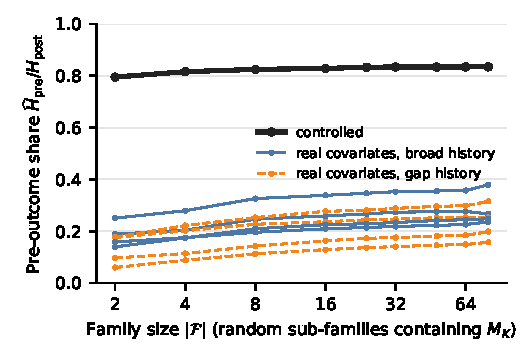
\includegraphics[width=0.62\linewidth]{figures/supplement_v5_family_size.pdf}
 \caption{包含 $M_K$ 的固定大小随机子族上，事后提升空间中的结果前占比（研究 E；128 个受控世界，每个真实协变量分支 64 对，全程使用相同的标签重复样本）。每条细线对应一个真实协变量分支。}
 \label{fig:family}
\end{figure}

\paragraph{常数与风险。}单独改变任一常数（分位数 $0.1$--$0.5$、惩罚 $0$--$0.44$、门限 $0$--$0.16$、衰减 $0$--$0.9$、tanh 尺度 $1.25$--$5$）对期望损失的影响至多 $1.3$，门限的影响从不超过 $0.03$。由于这些世界中 $p$ 已知，我们精确计算了所选集合实际不利敞口超过其包络的概率：对所有策略和状态都不超过 $2.8\times10^{-3}$，远低于 $\alpha=0.1$；尽管视策略不同，只有 95--99\% 的所选集合满足“全部成员 $q_i\ge p_i$”。

\section{真实协变量：机会去了哪里}
\label{sec:realx}
\paragraph{设计。}我们保留 HMEQ 与 LendingClub 的真实协变量，从已知的逻辑或非线性 logit（$p(x)=\sigma(-0.8+x^\top\beta)$，可选地加上 $0.5\sin x_2+0.35x_3x_4$）生成结果，从而可以度量 $H_{\mathrm{pre}}$。在每个设定的 64 对新样本中，一个 240 条记录的储备池提供两种历史：\emph{宽}（随机 80 条）与\emph{缺口}（第二个特征最低的 80 条）。两个分支的候选、待反馈与目标记录、标签、预处理、风险分数、预算、参照与候选族完全相同，因此配对只隔离历史覆盖的差别。

\paragraph{大部分事后提升空间是先见。}$H_{\mathrm{post}}$ 比受控世界小一个数量级，且大部分是先见（表~\ref{tab:realx}）：八个分支的结果前占比为 10--39\%（交叉拟合到插值），而每个受控变体中都是 82--88\%。两种场景的族大小相近（平均 22--23 对 27 个集合），且这一差距在每个匹配的族大小上都存在（图~\ref{fig:family}）：$|\mathcal F|=16$ 时真实协变量的占比为 13--34\%。把族扩大到 81--84 个集合，占比变化至多 6 个百分点；在随机子族上，占比随 $|\mathcal F|$ 略有上升而非下降，与“族大小造成的假象”恰好相反。从绝对量看，先见在各处相近：全部 21 个受控与真实协变量组中都在 $1.5$--$6.4$ 之间，而可部署部分从 $0.3$ 到 $41$ 不等。因此，当可行集合之间的真实差异与这一由标签噪声决定的 EVPI 同量级时（所有真实协变量分支都是如此），事后比较最具误导性。覆盖缺口使 $H_{\mathrm{post}}$ 翻倍以上（从 $1.9$--$2.4$ 升到 $4.9$--$6.4$），并使 $H_{\mathrm{pre}}$ 至多升到 $1.9$；九个组中先见都显著为正。

\begin{table}[t]
\caption{真实协变量状态（每个设定 64 对；$\times10^{-3}$ 期望 Brier）。$H_{\mathrm{pre}}$ 由交叉拟合与插值估计夹逼。“代理”为 $\arg\max_{\mathcal F}V_{\widehat\theta}$ 在评估族上的收益；$\rho$ 为 $V_{\widehat\theta}$ 与真实事前收益在 $\mathcal F$ 上的 Spearman 相关；“$=M_K$”为 DC-PRISM 返回参照的状态比例。}
\label{tab:realx}
\centering\small
\setlength{\tabcolsep}{2.5pt}
\begin{tabular}{llrrrrrr}
\toprule
设定 & 分支 & $H_{\mathrm{post}}$ & $H_{\mathrm{pre}}$ & DC 收益 & 代理收益 & $=M_K$ & $\rho$ \\
\midrule
HMEQ，逻辑 & 宽 & 2.19 & [0.48, 0.58] & 0.04 & 0.11 & 86\% & 0.27 \\
 & 缺口 & 6.37 & [1.49, 1.87] & $-0.04$ & 1.13 & 88\% & 0.64 \\
HMEQ，非线性 & 宽 & 2.43 & [0.85, 0.94] & $-0.02$ & 0.10 & 84\% & 0.31 \\
 & 缺口 & 5.83 & [1.51, 1.89] & 0.10 & 0.54 & 95\% & 0.55 \\
LC，逻辑 & 宽 & 2.00 & [0.29, 0.39] & 0.04 & 0.03 & 92\% & 0.33 \\
 & 缺口 & 4.88 & [0.51, 0.83] & 0.02 & 0.13 & 92\% & 0.69 \\
LC，非线性 & 宽 & 1.89 & [0.31, 0.41] & 0.01 & $-0.01$ & 88\% & 0.14 \\
 & 缺口 & 5.16 & [0.64, 0.96] & 0.04 & 0.05 & 95\% & 0.65 \\
\midrule
受控 & -- & 22.21 & [18.38, 18.53] & 12.19 & 10.69 & 4\% & $-0.01$ \\
\bottomrule
\end{tabular}
\end{table}

\paragraph{定位结果前差距。}DC-PRISM 在每个分支的事前收益都在 $\pm0.1$ 以内，因此它的选择差距几乎就是全部 $H_{\mathrm{pre}}$。分别在拟合参数 $\widehat\theta$ 与总体参数 $\theta_{\mathrm{pop}}$（真实 $p$ 在逻辑类上的 KL 投影）处按 $V_\theta$ 对评估族排序，在 16 项登记的真实协变量检验中，参数效应（均值 $0.02$--$0.61$）与剩余近似差距（$0.09$--$0.40$）都未达到实质水平。在覆盖缺口下代理对族的排序较好（$\rho=0.55$--$0.69$），其最大者在 HMEQ-逻辑中获得交叉拟合 $H_{\mathrm{pre}}$ 的 76\%，在其余缺口设定中只有 8--36\%。在受控世界中，代理对整个族的排序很差（$\rho\approx0$），其最大者却获得 $10.7$：它能识别少数最好的集合，但不能给其余集合排序。在受控世界中，按 $\theta_{\mathrm{pop}}$ 排序明显更差（$-11.2$ $[-15.7,-6.6]$），近似差距 $H_{\mathrm{pre}}^{\text{cf}}-\Gamma(\theta_{\mathrm{pop}})=18.4-(-0.5)=18.9$ $[14.2,23.5]$ 达到实质水平，与误设的尾部状态切换一致。

\paragraph{真实协变量上的保守层。}研究 F 的新消融重现了这一图景。DC-PRISM 在 86--98\% 的真实协变量状态中返回 $M_K$。在有覆盖缺口的 HMEQ-逻辑中，$\mathcal F^+$ 上的代理最大者相对参照收益 $1.40$ $[0.34,2.46]$，保守层放弃了其中的 $1.34$ $[0.38,2.30]$；其余七个分支中两者都在 $\pm0.65$ 以内，没有决定性的对比。结合受控消融，“保守有\emph{帮助}”的证据较弱（受控世界中未证实的 $+3.0$），而“在代理可靠处保守会\emph{损失}可部署价值”的证据更清楚，但只出现在八个分支中的一个。总的来说，真实协变量上涉及的量很小：在我们的设定中至多约 $2\times10^{-3}$ Brier 可部署。

\section{真实标签上的延迟回放}
\label{sec:replay}
\paragraph{协议。}我们在处理后的 HMEQ、LendingClub、PPDai 与 UCI Credit 队列上回放十轮，均使用 6 个特征与记录的二元结果~\cite{sasHMEQ,lendingclubSource,ppdaiSource,he2018ensemble,yeh2009comparison}。每个种子保留 1{,}000 条测试行、600 条目标行和一个 600 行的历史窗口，从中取 68 条初始记录。每轮提供 24 个候选与 14 个常规获取。探索标签在选择后一轮到达，常规标签在两轮后到达；每轮开始时、在到期标签释放之后度量 Brier、ROC-AUC 与 log-loss，并对十轮取平均（ALC）。预处理在初始历史上拟合，数值预算由初始模型确定并在各策略间固定。\emph{工程}流对可观测协变量排序，从较窄的初始历史出发提供低风险、与待反馈对齐、互补与尾部候选，模拟受控设计；\emph{自然}流随机抽取初始历史与每轮记录。DC-PRISM 与七个对照逐一比较，构成 56 项检验族。

\paragraph{功效。}此前每个队列 32 个种子的一批没有任何决定性比较，配对标准差为 $1.6$--$2.0$（自然流）与 $1.6$--$6.9$（工程流）$\times10^{-3}$。据此我们预先登记了每个队列每种流 512 个新种子；在这些标准差下，56 项 Bonferroni 校正、80\% 功效可检测自然流 $0.3$--$0.4\times10^{-3}$、工程流 $0.3$--$1.3\times10^{-3}$ 的差异。新一批中工程流的种子级配对标准差更大（$1.4$--$12.4\times10^{-3}$），因此其可检测效应最大到 $2.3\times10^{-3}$。

\begin{table}[t]
\caption{每个队列每种流 512 个新种子的延迟回放：平均 ALC-Brier（$\times10^{-2}$）与每轮平均标签数（“标签”）。种子级标准差为 $0.8$--$3.4\times10^{-2}$；差值在种子内配对。}
\label{tab:replay}
\centering\scriptsize
\setlength{\tabcolsep}{2.6pt}
\begin{tabular}{lrrrrrrrrr}
\toprule
& \multicolumn{4}{c}{工程流} & \multicolumn{4}{c}{自然流} & \\
\cmidrule(lr){2-5}\cmidrule(lr){6-9}
策略 & HMEQ & LC & PPDai & UCI & HMEQ & LC & PPDai & UCI & 标签 \\
\midrule
仅常规获取 & 17.57 & 17.78 & 13.09 & 17.51 & 13.65 & 15.79 & 11.74 & 15.80 & 0.0 \\
Safe-MinRisk & 17.61 & 17.54 & 12.96 & 17.49 & 13.56 & 15.68 & 11.63 & 15.64 & 6.8 \\
固定数量 & 17.59 & 17.54 & 12.89 & 17.49 & 13.56 & 15.67 & 11.63 & 15.63 & 5.5 \\
Random & 17.43 & 17.48 & 12.89 & 17.50 & 13.58 & 15.72 & 11.66 & 15.67 & 4.1 \\
Uncertainty & 17.41 & 17.65 & 12.72 & 17.50 & 13.58 & 15.70 & 11.61 & 15.64 & 3.9 \\
Fisher-cost & 16.99 & 17.17 & 12.73 & 17.49 & 13.51 & 15.65 & 11.61 & 15.62 & 4.4 \\
BAIT-greedy & 17.00 & 17.23 & 12.68 & 17.51 & 13.52 & 15.66 & 11.60 & 15.63 & 3.5 \\
TargetVar-greedy & 17.01 & 17.25 & 12.65 & 17.50 & 13.52 & 15.66 & 11.60 & 15.63 & 3.6 \\
DC-PRISM & 17.36 & 17.50 & 12.65 & 17.50 & 13.54 & 15.66 & 11.60 & 15.63 & 5.7 \\
\bottomrule
\end{tabular}
\end{table}

\begin{figure}[t]
 \centering
 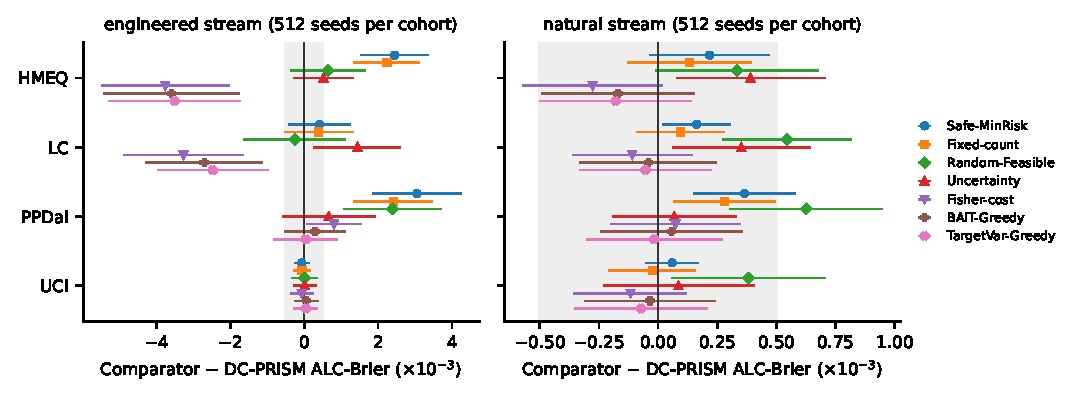
\includegraphics[width=\linewidth]{figures/supplement_v5_online.pdf}
 \caption{对照策略减 DC-PRISM 的 ALC-Brier，及 56 项检验族上的 95\% 同时区间（每格 512 个种子）；正值有利于 DC-PRISM。灰带：$\pm5\times10^{-4}$。注意两图横轴刻度不同。}
 \label{fig:replay}
\end{figure}

\paragraph{结果。}有了足够功效，回放给出了明确信息（表~\ref{tab:replay}、图~\ref{fig:replay}）。在工程流上，DC-PRISM 在 HMEQ（相对 Safe-MinRisk $2.4$、固定数量 $2.2$）与 PPDai（$3.1$、$2.4$，以及相对 Random $2.4$）上显著优于数量型参照，但在 HMEQ（$3.5$--$3.8$）与 LendingClub（$2.5$--$3.3$）上显著\emph{不如} Fisher-cost、BAIT-greedy 与 TargetVar-greedy，而这些策略所取标签更少、探索损失也更低；在 UCI Credit 上七项差异都落在实质带内。在自然流上没有任何比较达到实质水平：28 项中 19 项落在实质带内，另有 6 项以小于 $0.65$ 的幅度有利于 DC-PRISM（单位均为 $\times10^{-3}$）。作为次要检验族的 ROC-AUC 呈现相同格局：在工程流 HMEQ 上 DC-PRISM 比数量型参照高 $0.005$，在工程流 PPDai 上比 Random 与 Uncertainty 高 $0.010$--$0.015$，在工程流 LendingClub 上比 Fisher-cost 低 $0.005$；自然流上没有达到实质水平的 AUC 差异。在每个策略 40{,}960 个有采集的回合中，实际不利敞口超过包络的只有 0--4 次（DC-PRISM 为 2 次；Clopper--Pearson 上界 $\le2.2\times10^{-4}$），平均只占包络的 14--19\%。回放结果因此与第~\ref{sec:controlled}--\ref{sec:realx} 节一致：在真实结果上，考虑待反馈信息的比较在两个工程流队列上胜过“取最多标签”，但在另外两个队列上不如直接的信息贪心选择，而自然流无法区分各策略。

\paragraph{回放的有效性。}回放继承了公开信贷数据的两项局限。LendingClub（据我们所知其他队列也是如此）只包含已批准的贷款，因此“候选”来自已经筛选过的总体，被拒申请人的结果缺失~\cite{crook2004reject}；回放检验的是在此前可接受的申请人中进行获取，而非完整的选择性标签问题。数据按随机而非日历时间划分，一轮与两轮的延迟也是程式化设定。

\section{相关工作}
\label{sec:related}
\paragraph{信息价值与评价。}EVPI 与样本信息期望值是决策分析的经典概念~\cite{howard1966information,raiffa1961applied}；在带噪估计中挑选最优所产生的向上偏差被称为 optimizer's curse~\cite{smith2006optimizer}，或模型选择中的选择偏差~\cite{cawley2010overfitting}。Krause 与 Guestrin~\cite{krause2005near}在预算下优化信息价值。我们使用这些思想不是为了做选择，而是为了评价获取策略：先见项是可见族上的 EVPI，交叉拟合~\cite{chernozhukov2018double}提供夹逼的下侧。

\paragraph{实验设计与主动学习。}贝叶斯实验设计~\cite{chaloner1995bayesian}与主动学习~\cite{cohn1996active,settles2009active}通过选择观测来改进模型，准则从不确定性~\cite{lewis1994sequential}与转导式设计~\cite{yu2006transductive}，到 Fisher 信息~\cite{ash2021fishing}、梯度多样性~\cite{ash2020badge}、互信息~\cite{kirsch2019batchbald,bickfordsmith2023prediction}与决策损失~\cite{huang2026loss}；预算化变体处理异质成本~\cite{tomanek2010cost,morato2025conbatch}，背包约束下的子模最大化是贪心批量选择的基础~\cite{sviridenko2004note}。这些方法提供了我们使用的信息几何。

\paragraph{选择性标签、安全与延迟。}选择性标签研究刻画了只有有利决策才会揭示结果的情形~\cite{lakkaraju2017selective}；Wei~\cite{wei2021selective}、Kilbertus 等~\cite{kilbertus2020fair}与 Keswani 等~\cite{keswani2024partial}在探索与效用、公平或覆盖之间权衡，日志数据也可作为后续实验的起点~\cite{yan2018logged}。拒绝推断用于修正被拒申请人结果缺失的问题~\cite{crook2004reject}。安全探索~\cite{sui2015safe}、安全主动学习~\cite{schreiter2015safe}与保守 bandit~\cite{wu2016conservative}用安全性或基线要求约束探索；延迟反馈学习~\cite{joulani2013delayed,chapelle2014delayed}与延迟感知主动学习~\cite{pham2022latency}处理迟到的结果。

\section{讨论与结论}
\label{sec:conclusion}
与实现最优集合做事后比较，是论证某个选择规则“把价值留在了桌上”的自然方式。我们的协议说明了这种比较何时会误导。在围绕方向性待反馈信息构造的受控世界中，我们尝试的每种生成器变体里大部分事后提升空间都可部署，而在以参照为锚的族上评估的目标加权代理能以更少的标签获得其中很大一部分。先见本身是一个大致恒定的标签噪声下限，所以它的占比恰恰在真实差异小的地方大。在真实信贷协变量上，同样的提升空间大部分是 EVPI；可部署的剩余部分随覆盖缺口增大，并能被同一代理部分识别，但保守的决策规则基本没有利用它。在功效充足的真实结果回放中，同一规则在两个队列上胜过数量型参照，在另两个队列上不如信息贪心选择。对实践者而言，可操作的结论是这套协议本身：事后提升空间并不能很好地指示一个获取规则还能获得多少。

\paragraph{局限。}真实协变量上的结果由已知概率生成，因为度量 $H_{\mathrm{pre}}$ 需要它们。回放使用固定的、只含已批准贷款的处理后队列，并做随机划分，我们不声称完成了外部或时间外推验证。包络的概率保证需要 $q$ 的同时覆盖，我们的分数不能保证这一点，尽管实际超出远低于 $\alpha$。BAIT-greedy（只有前向步）与 TargetVar-greedy（EPIG 的 Laplace 近似）是适配版本，而非完整复现。常数是沿用而非推导得到的；扰动与敏感性研究限定了、但没有消除这一顾虑。

\paragraph{展望。}由此引出两个方向：评价获取规则时报告结果前而非事后提升空间；以及从可见信息诊断代理的可靠性，使保守性只在代理排序较差处施加。代码、带提交哈希的冻结协议、汇总结果与核验脚本见匿名仓库。

\bibliographystyle{splncs04}
\bibliography{refs}
\end{document}
